\chapter{Experiment\label{experiment}}

% TODO nějaký úvod, že ukazuju, jak je možné kombinovat OLAP a KG, co jsem použil za technologie, proč to dělám REPL

This section describes an experiment of mining associtation rules from RDF data compiled of statistical data structured by the Data Cube Vocabulary and facts pulled from the Wikidata data set that was performed as an practical part of this work. The statistical data come from two sources. The first one is the Czech Social Security Administration and the second one is the Czech Statistical Office. Analysis was performed using the Scala API of the reference implementation of the RDFRules algorithm. The following sections describe how the available data had to be preprocced to give reasonable results in combination with KG data. The preprocessing was perfomed partly by the implementation's API itself, partly by performing SPARQL queries over the data. The described method can be taken inspiration from when performing similar analysis ie. association rule mining task over the multidimensional data merged with loosely structured graph data. 

\section{Czech Social Security Administration's Data Cubes\label{cssa}}

Czech Social Security Administration (CSSA) is a czech public administration organtisation responsible for collecting social security premiums and contributions to the state employment policy. Since 2015 the organization publishes its statistical yearbook datasets and other (vocabularies, code lists and datasets containing data concerning the internal operation of the organization) in the form LOD and became one of the first czech public institutions to do so. The yearbook statistical data sets are modeled using Data Cube Vocabulary. Their dimension values are represented by the SKOS vocabulary. The organization has published 73 datasets so far. All these datasets are downloadable as dumps\footnote{\href{http://data.cssz.cz/web/otevrena-data/katalog-otevrenych-dat}{http://data.cssz.cz/web/otevrena-data/katalog-otevrenych-dat}} or accesible througth a SPARQL endpoint\footnote{\href{http://data.cssz.cz/web/otevrena-data/sparql-query-editor/}{http://data.cssz.cz/web/otevrena-data/sparql-query-editor/}}. The CSSA's URIs are dereferenceable.

% project vše
% že tam jsou i CSV data a pro každý data set je stránka s popisem

The largest of the data cubes published is \verb|cssa-d:duchodci-v-cr-krajich-okresech|\footnote{https://data.cssz.cz/resource/dataset/duchodci-v-cr-krajich-okresech}. From now on it will be denoted as \textit{Pensions}. It contains \numprint{368118} observations spread over four dimensions: reference area\footnote{https://data.cssz.cz/ontology/dimension/refArea}, reference period\footnote{https://data.cssz.cz/ontology/dimension/refPeriod}, sex\footnote{https://data.cssz.cz/ontology/dimension/pohlavi} and pension kind\footnote{https://data.cssz.cz/ontology/dimension/druh-duchodu}. Observations are assigned three measures: the average amount of pension\footnote{https://data.cssz.cz/ontology/measure/prumerna-vyse-duchodu-v-kc}, the average age\footnote{https://data.cssz.cz/ontology/measure/prumerny-vek} and the number of persons\footnote{https://data.cssz.cz/ontology/measure/pocet-duchodcu}. Each observation is assigned only one measure.

\begin{figure}[h]
\begin{lstlisting}[language = turtle, caption={Example of an observation from \textit{pensions} data set}, label={cssa1example},captionpos=b escapeinside={(*@}{@*)}]
@prefix qb: <http://purl.org/linked-data/cube#> .
@prefix cssa-om: <https://data.cssz.cz/ontology/measure/> .
@prefix cssa-d: <https://data.cssz.cz/resource/dataset/> .
@prefix cssa-od: <https://data.cssz.cz/ontology/dimension/> .

<https://data.cssz.cz/resource/observation/duchodci-v-cr-krajich-okresech/2017-12-31/prumerna-vyse-duchodu-v-kc/pk_srnvm/vc.35/m>
    a qb:Observation ;
    qb:dataSet cssa-d:duchodci-v-cr-krajich-okresech .
    qb:measureType cssa-om:prumerna-vyse-duchodu-v-kc ;
    cssa-od:druh-duchodu <https://data.cssz.cz/resource/pension-kind/PK_SRNVM_2010> ;
    cssa-od:pohlavi <https://data.cssz.cz/ontology/sdmx/code/sex-M> ;
    cssa-od:refArea <https://data.cssz.cz/resource/ruian/vusc/35>;
    cssa-od:refPeriod <https://data.cssz.cz/resource/reference.data.gov.uk/id/gregorian-day/2017-12-31>;
    cssa-om:prumerna-vyse-duchodu-v-kc 6622.0;
\end{lstlisting}
\end{figure}

In this particular data set there are \numprint{102} distinct values of the dimension of reference area: 14 regions (NUTS 3 administrative units, czech translation in singular nominative is \textit{kraj}) including Prague, 77 districts (\textit{okres}) also including Prague, 10 Prague districts (\textit{správní obvod}) and a value representing the state in total. Each entity representing a reference area is assigned an unique numerical identifier which corresponds to this area's identifier in the official Registry of Territorial Identification, Addresses and Real Estate (RTIAR) runned by the State Administration of Land Surveying and Cadastre (SALSC). RTIAR codes are reference codes by law, so it is obligatory for CSSA to use them and have them correct.

\begin{figure}[h]
\begin{lstlisting}[language = turtle, caption={Dereferenced proxy entity of the South Bohemian Region}, label={sbrexample},captionpos=b, escapeinside={(*@}{@*)}]
@prefix skos:  <http://www.w3.org/2004/02/skos/core#> .

<https://data.cssz.cz/resource/ruian/vusc/35>
    a <https://data.cssz.cz/ontology/ruian/Vusc> , skos:Concept ;
    <http://www.w3.org/2002/07/owl#sameAs> <https://linked.cuzk.cz/resource/ruian/vusc/35> ;
    skos:inScheme  <https://data.cssz.cz/resource/ruian/ConceptScheme> ;
    skos:notation "VC.35" ;
    skos:prefLabel "(*@Jihočeský kraj@*)" .
\end{lstlisting}
\end{figure}

There are official URIs of this registry but CSSA datasets do not use them directly. The~entities for the dimension of reference area and other dimensions in the dataset \textit{Pensions} and all other data sets of CSSA with the dimension of reference area work as so-called \textit{proxy entities}. This means that instead of using the original code list item URIs directly as objects in the RDF triples,  it uses their equivalents defined in the internal code lists. These equivalents are connected to the original URI by the \verb|owl:sameAs| statement. These proxies can then contain data specific to CSSA e.g. labels. Another advantage of this is, that these URIs are dereferenceable to the CSSA domain and their versioning is under the control of CSSA and they can be easily redirect to a different equivalent code list. Previously the proxy entities of the reference area were directed to the unofficial transformation of the Opendata.cz initiative\footnote{\href{https://linked.opendata.cz/dataset/cz-ruian}{https://linked.opendata.cz/dataset/cz-ruian}}.

Another dimension whose values work as proxy entities is the dimension of reference period. This dimension divides the observations into one year intervals. This applies to all other CSSA data cubes containg the reference period dimension. The data set vary in the overall covered period. The first covered time period is the year 2001 and the last covered year of all data sets is the year 2019. The entities link to the \verb|data.gov.uk| Time Intervals\footnote{\href{http://old.datahub.io/dataset/data-gov-uk-time-intervals}{http://old.datahub.io/dataset/data-gov-uk-time-intervals}} OWL ontology. Usage of this entities is, however, not unified. In some data sets intervals are assigned an entity representing a year, in other they are assigned an entity representing the last day of the corresponding year. All of them are, however, representing a period of a whole year.

\begin{figure}[h]
\begin{lstlisting}[language = turtle, caption={Dereferenced proxy entity of the year 2017}, label={gd2017example},captionpos=b, escapeinside={(*@}{@*)}]
@prefix skos:  <http://www.w3.org/2004/02/skos/core#> .

<https://data.cssz.cz/resource/reference.data.gov.uk/id/gregorian-year/2017>
    a skos:Concept ;
    <http://www.w3.org/2002/07/owl#sameAs> <http://reference.data.gov.uk/id/gregorian-year/2017> ;
    skos:inScheme <https://data.cssz.cz/ontology/years/YearsScheme> ;
    skos:notation "2017" ;
    skos:prefLabel "2017" .
\end{lstlisting}
\end{figure}

The \textit{Pensions} dataset uses two distinct schemes for the pension kinds, because in 2010, the official categorization of pensions was changed in the czech legislation. Only the observations assigned to year 2008 are divided according to the old pension scheme. All other year's observations correnspond to the new pension scheme. So one can not simply multiply the numbers of distinct values for each dimension and the number of measures to get the total number of observations for this particular cube. The URIs of both pension kind schemes are suffixed either by \verb|_2008| (31 of them) for the old scheme or \verb|_2010| (37 of them) for the new scheme. Not all entities correspond to a particular kind of pension. Some of them represent an aggregation over related pension kinds or simply an aggregation over all of the pension kinds.

\begin{figure}[h]
\begin{lstlisting}[language = turtle, caption={Dereferenced pension kind}, label={pkexample},captionpos=b, escapeinside={(*@}{@*)}]
@prefix skos:  <http://www.w3.org/2004/02/skos/core#> .

<https://data.cssz.cz/resource/pension-kind/PK_SRNVM_2010>
    a <https://data.cssz.cz/ontology/pension-kinds/PensionKind> , skos:Concept ;
    skos:altLabel "SRNVM"@cs ;
    skos:exactMatch <https://data.cssz.cz/resource/pension-kind/PK_SRNVM> ;
    skos:inScheme <https://data.cssz.cz/ontology/pension-kinds/PensionKindScheme_2010> ;
    skos:notation "PK_SRNVM" ;
    skos:prefLabel "(*@Starobní důchod SRN vyplácený v souběhu s vdoveckým důchodem@*)"@cs .
\end{lstlisting}
\end{figure}

The dimension of sex consists of three distinct values: dimension of male pension, dimension of female pensions and a value for both sexes. The values are proxy entities as well linking to the SDMX representations of sexes\footnote{\href{http://purl.org/linked-data/sdmx/2009/code}{http://purl.org/linked-data/sdmx/2009/code}}

\section{Czech Statistical Office's Data Cubes}

The Czech Statistical Office (CZSO) is the main public organization responsible for collecting and analyzing statistical data in the Czech Republic. This organization is for example responsible for the state's census. Data about demography, economics, education, health care, etc. are made availabe on the organization's website\footnote{\href{https://vdb.czso.cz/vdbvo2/faces/en/index.jsf?page=uziv-dotaz}{https://vdb.czso.cz/vdbvo2/faces/en/index.jsf?page=uziv-dotaz}} in a form of interactive spreadsheet builder. Thanks to the Opendata.cz initiative this data sets are made available as LOD modelled by the Daca Cube Vocabulary in the initiative's catalogue. The data is also hosted as a SPARQL endpoint\footnote{\href{http://linked.opendata.cz/sparql}{http://linked.opendata.cz/sparql}}. 8 of these data sets have a dimension of reference period. Each data set’s dump file can be downloaded from the catalouge\footnote{The download link URLs are, however, broken and return HTTP status code 404. To get the dump file, word \textit{dumps} has to be substituted with word \textit{soubor} (czech word for \textit{file}). For example, the dump file of the data set \textbf{czso-job-applicants} is available at \href{https://linked.opendata.cz/soubor/czso-job-applicants.trig}{https://linked.opendata.cz/soubor/czso-job-applicants.trig}}.

\begin{figure}[h]
\begin{lstlisting}[language = turtle, caption={Example of an observation from the CZSO data sets}, label={turtleexample},captionpos=b escapeinside={(*@}{@*)}]
@prefix qb: <http://purl.org/linked-data/cube#> .
@prefix czso: <http://data.czso.cz/ontology/> .

<http://data.czso.cz/resource/observation/job-applicants-and-unemployment-rate/CZ0513/2009-12-31/T> a qb:Observation ;
    czso:refArea <http://ruian.linked.opendata.cz/resource/okresy/3505> ;
    czso:refPeriod <http://reference.data.gov.uk/id/gregorian-day/2009-12-31> ;
    czso:sex sdmx-code:sex-T ;
    czso:neumisteniUchazeciOZamestnani 9692.0 ;
    czso:dosazitelniNeumisteniUchazeciOZamestnani 9528.0 ;
    czso:podilNezamestnanych 7.92 ;
    czso:pocetVolnychMist 569.0 ;
    qb:dataSet <http://data.czso.cz/resource/dataset/job-applicants-and-unemployment-rate> .
\end{lstlisting}
\end{figure}

Observations in CZSO data cubes are assigned multiple measures. Their URIs are not dereferenceable. Their dimension value URIs do not work as proxy entities. The dimension of reference area uses entities of an above-mentioned initiative's unofficial RTIAR transformation\footnote{\href{https://linked.opendata.cz/dataset/cz-ruian}{https://linked.opendata.cz/dataset/cz-ruian}} with its own SPARQL endpoint\footnote{\href{https://ruian.linked.opendata.cz/sparql}{https://ruian.linked.opendata.cz/sparql}}. The measured values relate to regions and district. They do not contain observations related to the whole state. The proxy entities of the reference area dimension values for the CSSA data sets previously linked to this code list. 

For time intervals representation the CZSO data cubes also use the \verb|data.gov.uk| Time Intervals OWL ontology. They only do so directly unlike the CSSA data cubes. The data cubes vary in their time span. The earliest recorded values are for the year 2005. The latest values are for the year 2013. There are two data sets that contain values for both the earliest and latest year mentioned meaning they cover a period of 9 years: \textbf{czso-deaths-by-selected-causes-of-death}\footnote{\href{https://linked.opendata.cz/dataset/czso-deaths-by-selected-causes-of-death}{https://linked.opendata.cz/dataset/czso-deaths-by-selected-causes-of-death}} and \textbf{czso-job-applicants-and-unemployment-rate}\footnote{\href{https://linked.opendata.cz/dataset/czso-job-applicants-and-unemployment-rate}{https://linked.opendata.cz/dataset/czso-job-applicants-and-unemployment-rate}}

Just as with the CSSA data cubes, some of the CZSO data cubes contain the dimension of sex consisting of three distinct values: dimension of male pension, dimension of female pensions and its total. The values used are the SDMX representations of sexes themselves.

\section{Wikidata}

Wikidata data set also contains data about political representation of countries, their administrative areas and municipalities. For the purposes of this experiment, such data concerning the Czech Republic was extracted from the data set. In the Czech Republic, regions and municipalities\footnote{Not districts though.} are being assigned a government that emerges from elections. In Wikidata data set, there exist records of who was or still is head of this local government, including the head of the state government. Records of these \textit{head of government} roles are given a time period of validity of this role by stating the date of this role's start and optionally the end of this role when it is not a current area government head anymore. For the persons who hold or held the office, the affiliation to a political party is stated in the data also with the start and end date of this affiliation. The entities of the political parties are assigned their political alignment (left, center, far-right, etc.). In the sample of Wikidata data set's content below it is stated that since 2008 till 2016 the head of the government of the South Moravian Region was Michal Hašek who since 1998 is a member of the Czech Social Democratic Party, which has the centre-left political alignment.

\begin{figure}[h]
\begin{lstlisting}[language = turtle, caption={Deluge of Wikidata triples}, label={wdhasekexample},captionpos=b, escapeinside={(*@}{@*)}]
@prefix wd: <http://www.wikidata.org/entity/> .
@prefix p: <http://www.wikidata.org/prop/> .

wd:Q192697 rdfs:label "South Moravian Region"@en ;
    p:P6 [ p:P6 wd:Q6835752 ; p:P580 "2008-11-21T00:00:00Z" ; p:P582 "2016-11-16T00:00:00Z" ] .

wd:Q6835752 rdfs:label (*@"Michal Hašek"@*)@en ;
    p:P102 [ p:P102  wd:Q341148 ; p:P580 "1998-01-01T00:00:00Z" ] .

wd:Q341148 rdfs:label "Czech Social Democratic Party"@en ;
    p:P1387 [ p:P1387 wd:Q737014 ] .

wd:Q737014 rdfs:label "centre-left"@en .
\end{lstlisting}
\end{figure}

When adequately preprocced, this data can be utilized to find relations of statistical data described in the data cubes of CSSA and CZSO and the political cycle in the country. For example a rule can be found that states, that if in any year, the head of the Czech Republic's government was a member of a left-leaning policital party, the pension expenses for one-off allowance to pensions were above average. A query that extracts this data from the Wikidata's SPARQL endpoint is listed in \ref{wdextract}. This data, however, cannot be used for mining such rules yet. Measures in the data cubes are recorded on year to year bases. For the governmental roles and political affiliations it is only know the start date and end date. It is necessary to transform these triples into set of triples stating that a governmental role or the policital affiliation \textit{applies} for a certain year. The edge years are a bit tricky because the role or the membership was not valid for the whole year it started or ended. To facilitate the query and to generate more triples I decided to generate the triples for the edge years as well. The SPARQL query that constructs the \textit{appliesToRefPeriod} triples from the extracted data is listed in \ref{wdapplies}. The triples stating the start dates and end dates are no longer needed and do not have to be loaded into the RDFRules mining task.

The triples with predicates of \verb|p:P582| and \verb|p:P580| are no longer needed and are filtered out during the preproccesing. That will leave the data with \numprint{24410} distinct triples.

\section{YAGO Triples}

Triples concerning the entitities of reference areas in the examined data cubes can also be found in the YAGO\footnote{\href{https://yago-knowledge.org/}{https://yago-knowledge.org/}} dataset, which extracts facts about real world entities from various sources (Wikipedia, GeoNames, WordNet, etc.). For a change unlike with the Wikidata dataset, for the experiments involving the this data the needed triples are not extracted according to a rigidly structured CONSTRUCT queries but with loose DESCRIBE queries returning all triples concerning the sought entities. The used queries\footnote{\href{https://github.com/nvkp/diploma-thesis-code/tree/master/data/yago}{https://github.com/nvkp/diploma-thesis-code/tree/master/data/yago}} extract the triples containing the reference areas themselves, the entities appearing in the triples together with the reference area entities (\textit{hop~1}) and the entities appearing in the triples of those entities (\textit{hop 2}). YAGO's public SPARQL endpoint's web interface\footnote{\href{https://yago-knowledge.org/sparql}{https://yago-knowledge.org/sparql}} has trouble handling the volume of the triples returned in the latter mentioned queries so one is better off quering the endpoint directly through a HTTP client.

Both districts and regions of the Czech Republic have their class\footnote{\href{http://yago-knowledge.org/resource/Districts\_of\_the_Czech\_Republic}{http://yago-knowledge.org/resource/Districts\_of\_the\_Czech\_Republic}}\footnote{\href{http://yago-knowledge.org/resource/Regions\_of\_the\_Czech\_Republic}{http://yago-knowledge.org/resource/Regions\_of\_the\_Czech\_Republic}} of which they are subclass in the YAGO dataset so the needed triples are easy to query. Total of \numprint{2992361} distinct triples was extracted, containing data about persons connected to the areas, geographical information about the areas (for example which region contains which district), etc.

\begin{figure}[h]
\begin{lstlisting}[language = turtle, caption={Example of the Extracted YAGO Triples}, label={yagoexample},captionpos=b, escapeinside={(*@}{@*)}]
@prefix schema: <http://schema.org/> .
@prefix yago: <http://yago-knowledge.org/resource/> .

yago:Prague a yago:Capital_city .
yago:Josef_Ji(*@ří@*)_Stankovsk(*@ý@*)_Q12026167 schema:deathPlace yago:Prague .
yago:What_the_Old_Man_Does_is_Always_Right_Q13564487 schema:translator yago:Josef_Ji(*@ří@*)_Stankovsk(*@ý@*)_Q12026167
\end{lstlisting}
\end{figure}

Around 62\% of the extracted triples are not relevant for the performed tasks. Their objects are literals (\verb|rdfs:label|, \verb|rdfs:comment| and \verb|schema:alternateName|) or image URLs (\verb|schema:image|). These triples are filtered out before the index data structure is constructed.

\section{Filtering the Observations}

The values for the city of Prague are duplicated. The city is assigned an entity both as a region and as a district. The administrative area of the Czech Republic's capital is given a special status by the Act No. 131/2000 Coll., on the Capital City of Prague and does not in fact fall into neighter of those categories. Nonetheless, Prague is assigned an identifier both as a district (\numprint{3100}) and as a region (\numprint{19}) in the RTIAR registry. When it comes to total population of the area (\numprint{1324227} as of 2020), it is comparable to other czech regions. The least populated is the Karlovy Vary Region with around \numprint{300000} inhabitants and the most populated: the Central Bohemian Region has around \numprint{1300000} inhabitants. Its surface area is on the other hand comparable with the districts. As the statistics about pensioners are certainly more correlated with the population rather than the surface area, the observation allocated to the dimension value of Prage as being district would be filtered out to maintain the commensurability along values measured for districts (see \ref{cssaSlicing}).

I also chose to filter out all observations regarding year 2008. For 2008 the pension kinds are structured according to a different scheme than any other year and it is hard to assume compatibility for the URIs that only differ in the year's suffix. 2008 scheme contains penkind kinds that 2010 does not end vice versa. It could be possible to just cut the cube so that the year's 2008 become one cube and the other years the other one, but a cube concerning only one reference period has not got much value. Both filters can be performed in a single SPARQL query. In the \textit{Pensions} data set, discarting the Prague as a District entity removes \numprint{3609} observations. The year 2008 contained \numprint{28458} observations. \numprint{336330} observations are contained in the query's result making up 91,4\% of the unfiltered data set.

\begin{figure}[h]
\begin{lstlisting}[language = SPARQL, caption={SPARQL query to filter the \textit{Pensions} data set}, label={sparqlexample},captionpos=b escapeinside={(*@}{@*)}]
PREFIX skos: <http://www.w3.org/2004/02/skos/core#>
PREFIX qb: <http://purl.org/linked-data/cube#>
PREFIX cssa-d: <https://data.cssz.cz/resource/dataset/>
PREFIX cssa-od: <https://data.cssz.cz/ontology/dimension/>
PREFIX cssa-rd: <https://data.cssz.cz/resource/ruian/okresy/>
PREFIX cssa-op: <https://data.cssz.cz/ontology/pension-kinds/>

CONSTRUCT {
    ?observation ?p ?o
} 
WHERE {
    GRAPH cssa-d:duchodci-v-cr-krajich-okresech {
        ?observation qb:dataSet cssa-d:duchodci-v-cr-krajich-okresech ;
            cssa-od:druh-duchodu ?druh ;
            ?p ?o .
        NOT EXISTS {
            ?observation cssa-od:refArea cssa-rd:3100 .
        }
     }
     GRAPH cssa-d:pomocne-ciselniky {
        ?druh skos:inScheme cssa-op:PensionKindScheme_2010 .
     }
}
\end{lstlisting}
\end{figure}

\section{Slicing the Cubes\label{cssaSlicing}}

It is aimed to mine rules, in which the head atom's predicate is one of the cube's measures. In order to ensure, that such rules can achieve a reasonable support, the numerical values at the position of object in the measure triples have to be discretized and replaced by intervals. Irrespective to a chosen discretization approach, it is inadmissible to discretize values belonging to different disproportionate contexts (see \ref{commensurability}). For example, we cannot create intervals for the number of pensioners from values measured for both regions and districts together. A district is a lower administrative unit. It belongs to a lower level in the concept hierarchy and it is assumed that its numbers of pensioners are of a different order of magnitude than those for regions or for the whole state. Same applies for values of dimensions sex and pension kind of the described data set. The values of the reference period represent even time intervals so the commensurability is assumed.

The chosen way to solve this is to slice the preprocessed cubes having disproportionate dimension values into sets of smaller subcubes, in which the dimension values belong to the same level of a concept hierarchy. Measured values were then discretized into intervals in each subcube separately. Also when the commensurability could not be expected among dimension values on the same level of their hierarchy, A cut was made for each dimension value. For example the \textit{Pensions} data set had to be divided into 333 subcubes. It has 37 pension kinds. Dimension of sex has three distinct values: each sex and total. The dimension of reference area is considered to have 3 hierarchy levels: State's total, regions and Prague districts combined with the regional districts since they are comparable in number of inhabitants.

$$
37 \times 3 \times 3 = 333\hspace{0.4em}subcubes
$$

The dataset \verb|cssa-d:vydaje-na-duchody-v-cr|\footnote{\href{https://data.cssz.cz/resource/dataset/vydaje-na-duchody-v-cr}{https://data.cssz.cz/resource/dataset/vydaje-na-duchody-v-cr}} capturing costs on pensions in the Czech Republic by year and kind of pension contains 10 distinct values of the dimension of pension kind (not considering the scheme used only for year 2008). The cube had to be divided into 10 subcubes for each value of the pension kind dimension.

The construction of a subcube from a \textit{master} cube can be performed by a SPARQL CONSTRUCT query. An example of such query is shown in the listing \ref{sparqlcutexample}. This query filters the triples of the CZSO data cube \textbf{czso-job-applicants-and-unemployment-rate} to create a smaller cube of statistics about job applicants and unemployment rate for districts by sex. Notice how the reference area values corresponding to districts are distinguished. After the reference area values are linked (see \ref{linking}) to their CSSA counterparts, the ontology provided with the CSSA data sets can be reused.

\begin{figure}[h]
\begin{lstlisting}[language = SPARQL, caption={SPARQL query to create a subcube}, label={sparqlcutexample},captionpos=b escapeinside={(*@}{@*)}]
PREFIX qb: <http://purl.org/linked-data/cube#>
PREFIX sdmx-c: <http://purl.org/linked-data/sdmx/2009/code#>
PREFIX czso: <http://data.czso.cz/ontology/>
PREFIX czso-rd: <http://data.czso.cz/resource/dataset/>
PREFIX cssa-rd: <https://data.cssz.cz/resource/dataset/>
PREFIX cssa-or: <https://data.cssz.cz/ontology/ruian/>
PREFIX owl: <http://www.w3.org/2002/07/owl#>
    
CONSTRUCT { ?observation ?p ?o } 
WHERE { 
    GRAPH czso-rd:job-applicants-and-unemployment-rate {
        ?observation qb:dataSet czso-rd:job-applicants-and-unemployment-rate ;
            ?p ?o ;
            czso:refArea ?refAreaCZSO .
        NOT EXISTS {
            ?observation czso:sex sdmx-c:sex-T .
        }             
     }
    ?refAreaCSSZ owl:sameAs   ?refAreaCZSO.
    GRAPH cssa-rd:pomocne-ciselniky { ?refAreaCSSZ a cssa-or:Okres }
}
\end{lstlisting}
\end{figure}

For every subcube a similar query has to be created and performed over the master cube. For a cube that has to be divided into a small number of subcubes it is plausible to write (and save it for the documentation and repeatability purposes) and perform these queries manually. But there are cubes for which this would involve an hours long work. At the same time, it is an trivial activity that can easily be automated. For this preproccesing step for the \textit{Pensions} dataset, a Scala script\footnote{\href{https://github.com/nvkp/diploma-thesis-code/blob/master/data/pensions/script.scala}{https://github.com/nvkp/diploma-thesis-code/blob/master/data/pensions/script.scala}} was written that creates 333 distinct SPARQL queries that construct 333 subcubes, saves each query to a text file and also creates a shell script that triggers all queries and saves a result of each query to a distinct file in the turtle format. This, however, still requires writing such script for each preprocced data cube and solve the problem of a time consuming resolution of the queries.

The URIs of the data set to which the observations pointed with the $qb:dataSet$ had to be change to a \textit{subcube specific} URI so that the observations in a rule can be anchored to a single subcube for a variable.


\section{Linking\label{linking}}

In order to find rules describing relations across multiple sources (meaning data cubes of CZSO, data cubes of CSSA, Wikidata and YAGO triples) the entities either have to be assigned the same URIs or to be connected by the \verb|owl:sameAs| statements. The shared dimensions of the CSSA and CZSO data cubes are the reference area, reference period and sex. The dimension values URIs used for these dimensions differ not only institution from institution but also data cube from data cube from the same institution (In the CSSA data cubes, reference period is represented by an entity of a year and of the last day of the year as well). Linking of equivalent dimension values of the three dimensions is done by creating \verb|owl:sameAs| statements.

\subsection{Sex Dimension Values}

It was already mentioned that the CSSA data cubes use proxy entities linking to the SDMX representations of sexes, whereas the CZSO data cubes use these representations directly. So the linking statements are already provided with the CSSA code list file. To extract these very triples, the query listed below can be used. These triples can be than loaded into a mining task involving mining from data cubes contain the dimension of sex instead of loading the whole code list file.

\begin{figure}[h]
\begin{lstlisting}[language = SPARQL, caption={Linking the sex dimension values}, label={sexlinkextract},captionpos=b, escapeinside={(*@}{@*)}]
PREFIX owl: <http://www.w3.org/2002/07/owl#>

CONSTRUCT { ?cssaSex owl:sameAs ?sdmxSex }
WHERE {
    GRAPH <https://data.cssz.cz/resource/dataset/pomocne-ciselniky> {
        ?cssaSex a <https://data.cssz.cz/ontology/sdmx/code/Sex> ; owl:sameAs ?sdmxSex
    }
}
\end{lstlisting}
\end{figure}

\subsection{Reference Periods}

In CSSA data cubes, values from two concept schemes are used for representing the year intervals: a years scheme and a days scheme. The entities in the schemes are proxy entitities linking to the \verb|data.gov.uk| Time Intervals ontology. CZSO data cubes use the ontology's day scheme concepts directly. That means that every year is represented by three distinct URIs in the data cubes so two \verb|owl:sameAs| statements are required for each year. A query was written that generates these statements for every year entity in the CSSA code list:

\begin{figure}[h]
\begin{lstlisting}[language = SPARQL, caption={Linking the reference periods}, label={refperiodlinking},captionpos=b, escapeinside={(*@}{@*)}]
PREFIX owl: <http://www.w3.org/2002/07/owl#>
PREFIX skos: <http://www.w3.org/2004/02/skos/core#>
    
CONSTRUCT {
    ?cssaYear owl:sameAs  ?cssaDay .
    ?cssaYear owl:sameAs ?dataGovDay .
    ?cssaDay owl:sameAs ?dataGovDay .
}  
WHERE {
    GRAPH <https://data.cssz.cz/resource/dataset/pomocne-ciselniky> {
        ?cssaYear skos:inScheme <https://data.cssz.cz/ontology/years/YearsScheme>
        BIND (REPLACE(str(?cssaYear),".*(\\d{4})","$1") as ?cssaYearValue)
        ?cssaDay skos:inScheme <https://data.cssz.cz/ontology/days/DaysScheme>
        FILTER (REGEX(str(?cssaDay), ".*day.*12-31"))
        BIND (REPLACE(str(?cssaDay),".*(\\d{4})-12-31","$1") as ?cssaDayValue)
        ?cssaDay owl:sameAs ?dataGovDay
        FILTER (?cssaYearValue = ?cssaDayValue)
    }
}
\end{lstlisting}
\end{figure}

\subsection{Reference Areas}

The proxy entities of the reference area in CSSA data set used to link to the same entities that are used by the CZSO data sets. This linking is no longer present in the CSSA's code list but can be retrieved from the Opendata.cz's SPARQL endpoint. The query listed below returns 114 linking triples for all districts (including the Prague district entity), all regions (including Prague), Prague districts and the entity of the whole state.

\begin{figure}[h]
\begin{lstlisting}[language = SPARQL, caption={Linking the reference areas of CSSA and CZSO}, label={refarealinking},captionpos=b, escapeinside={(*@}{@*)}]
PREFIX owl: <http://www.w3.org/2002/07/owl#>

CONSTRUCT {
    ?cssaArea owl:sameAs ?odArea
}
WHERE {
    ?cssaArea a ?class ; owl:sameAs ?odArea .
    FILTER (?class IN (
        <https://data.cssz.cz/ontology/ruian/Okres>,
        <https://data.cssz.cz/ontology/ruian/Vusc>,
        <https://data.cssz.cz/ontology/ruian/SpravniObvod>,
        <https://data.cssz.cz/ontology/ruian/Stat>
        )
    )
}
\end{lstlisting}
\end{figure}

The linking with the Wikidata's entities had to be performed manually. But the YAGO data set already contains the $owl:sameAs$ triples linking to Wikidata, so it was easy to extract those triples by a second SPARQL query and \textit{close the linking circle}.

\begin{figure}[h]
\begin{lstlisting}[language = SPARQL, caption={Linking the reference areas of YAGO and Wikidata}, label={refarealinking},captionpos=b, escapeinside={(*@}{@*)}]
PREFIX owl: <http://www.w3.org/2002/07/owl#>
PREFIX yago: <http://yago-knowledge.org/resource/>
PREFIX schema: <http://schema.org/>
    
construct {
?region owl:sameAs ?sameRegion .
?district owl:sameAs ?sameDistrict .
}
where {
    ?region a yago:Regions_of_the_Czech_Republic .
    OPTIONAL {
        ?region schema:containsPlace ?district.
        ?district a yago:Districts_of_the_Czech_Republic .
        ?district owl:sameAs ?sameDistrict .
        FILTER REGEX(str(?sameDistrict), ".*http://www.wikidata.org/entity/.*")
    } 
    
    ?region owl:sameAs ?sameRegion .  
    FILTER REGEX(str(?sameRegion), ".*http://www.wikidata.org/entity/.*")
}
\end{lstlisting}
\end{figure}

\section{Discretization\label{discretization}}

Only the equifrequent discretization was chosen for the purposes of this experiment. Multiple discretizations (different interval counts) were performed with different parameters. If the sizes of the subcubes varied a lot, different sets of discretizations (interval counts) were set for them, because very coarse intervals worked fine for smaller subcubes, but with the same intervals the number of rules generated from the bigger subcubes was too high to be worked with even when the timeout threshold was set.

\section{Mining Tasks}

The source codes of the performed experiment are available in repository on github\footnote{\href{https://github.com/nvkp/diploma-thesis-code}{https://github.com/nvkp/diploma-thesis-code}} in the directory \textit{notebooks} in a form of jupyter\footnote{\href{https://jupyter.org/}{https://jupyter.org/}} notebooks. A Scala kernel for jupyter (eg. \textit{almond.sh}\footnote{\href{http://almond.sh/}{http://almond.sh/}}) has to be install in order to execute the code directly from the notebooks (see \textit{README.md}). Some of the notebooks are dedicated to preproccesing of a particular data set and other contain the performed mining tasks. In the preproccesing notebooks the preprocced data set is exported to a text file in the \textit{Turtle} format and also saved into a cache file from which the data set is loaded into memory before a mining task.  Github strictly enforces 100 MB size limit for each file so the cache files and \textit{Turtle} files are not pushed into the repository. In order to run the mining tasks locally one has to create the cache files by running the code in the preproccesing notebooks.

\subsection{Relation between the pension expenses and the policital alignment of the state's government\label{expenses-wikidata}}

A relation can be assumed between the expenditure on pensions in a state social security system and the political ideology of the state. A left leaning governments usually tend to spend more on social welfare than the right-wing governments. In this section it is shown how this relation can be described by association rules in the spirit of \ref{asocRule} mined from the data published by CSSA and Wikidata. Data from various countries would be more appropriate for mining such relation. The available data are, however, sufficient for a simple demonstration. 

The data cube used\footnote{\href{https://data.cssz.cz/web/otevrena-data/-/vydaje-na-duchody-v-cr}{https://data.cssz.cz/web/otevrena-data/-/vydaje-na-duchody-v-cr}} is published by CSSA and contains records of total annual expenses on particular pensions. From now on it will be denoted as \textit{expenses}. The only measure of the data cube is the expenditure amount in thousands of CZK. The dimensions of the data cube are the reference period with the granularity of whole years (from 2008 till 2019) and the dimension of the pension kind containing individual pension kind and also aggregated dimension values. For the year 2008 and 2009 and old pension scheme is used so the observations considering these two years were discarded. For the dimension of reference period 10 distinct values remain and the newer pension kind scheme contains also 10 distinct values. That would suggest that 100 observations remain but there are only 94. For the one-off allowance to pensions there are only 4 observations. That probably means that the expenses for this pension kind in the missing years were zero. So the missing observations with the measured value of zero were created manually.

The original data cube was sliced into 10 subcubes (by SPARQL queries) each containing 10 observations. Each subcube is in a separate file in the folder \verb|data/expenses|. In the notebook \verb|expenses.ipynb|\footnote{\href{https://nvkp.github.io/diploma-thesis-code/notebooks/expenses}{https://nvkp.github.io/diploma-thesis-code/notebooks/expenses}} each subcube's measures are discretized equifrequently (with 2 and 5 intervals) and equisizeably (with the relative support of 20, 30 and 50 percent) assigning each measurement 5 intervals.

The preproccesing of the Wikidata data set (notebook \verb|wikidata.ipynb|\footnote{\href{https://nvkp.github.io/diploma-thesis-code/notebooks/wikidata}{https://nvkp.github.io/diploma-thesis-code/notebooks/wikidata}}) rested in merging the triples returned by queries \ref{wdextract} and \ref{wdapplies} and removing the triples with predicates \verb|P580| and \verb|P582| as they only served to generate derived triples in the query \ref{wdapplies}.

In the notebook (\verb|expenses-wikidata.ipynb|\footnote{\href{https://nvkp.github.io/diploma-thesis-code/notebooks/expenses-wikidata}{https://nvkp.github.io/diploma-thesis-code/notebooks/expenses-wikidata}}) of the mining task the two preprocessed data sets were loaded and merged together with the reference period linking triples. From this data set containing \numprint{25494} triples an instance of index was created. The rules that should be found are described in plain text as \textit{If in any year the current prime minister belongs to a political party that has a certain political alignment then the annual expenses of a certain pension kind fit into certain interval}. 

Let's write it as a \textit{pseudo} rule pattern in the context of the available data's structure:
$$
(?headRole\hspace{0.4em}appliesTo\hspace{0.4em}?refPeriod) (\langle Czech\_Republic\rangle\hspace{0.4em}headOfGovernment\hspace{0.4em}?headRole) 
$$
$$
\land (?headRole\hspace{0.4em}person\hspace{0.4em}?person) \land (?person\hspace{0.4em}partyRole\hspace{0.4em}?partyRole) 
$$
$$
\land (?party\hspace{0.4em}alignment\hspace{0.4em}AnyConstant) \land (?partyRole\hspace{0.4em}party\hspace{0.4em}?party) 
$$
$$
\land (?partyRole\hspace{0.4em}appliesTo\hspace{0.4em}?refPeriod) \land (?observation\hspace{0.4em}refPeriod\hspace{0.4em}?refPeriod)
$$
$$
\land (?observation\hspace{0.4em}dataSet\hspace{0.4em}AnyConstant) \Rightarrow (?observation\hspace{0.4em}expenses\hspace{0.4em}AnyConstant)
$$

The variable $?headRole$ would be instantiated by entities representing an acting of a specific person in the office just as the variable $?partyRole$ would be instantiated by entities of memberships of a specific person in a specific political party. The rules yielded from this rule pattern would differ only by the entities at the object positions of the fifth and nineth atom and the head atom. The last body atom with the \verb|qb:dataSet| will ensure that all $?observation$ bindings belong to the same sub cube and thus the commensurability of measures will be preserved. There is no need of an atom stating the pension kind, because all observations in a sub cube share the same one. That way the rule is shorter.

The used algorithm implementation does not allow custom names for variables in a pattern. The variable names have to be single characters ordered alphabeticaly beginning with $?a$ from the rule's head. The definition of the rule pattern object to match the sought relations in this mining task is shown in listing \ref{alignmentExpensesPattern}:

\begin{figure}[h]
\begin{lstlisting}[language = scala, caption={First pattern definition}, label={alignmentExpensesPattern},captionpos=b, escapeinside={(*@}{@*)}]
val alignmentExpenses: RulePattern = (
    AtomPattern(subject = 'f', predicate = appliesTo, `object` = 'b') &:
    AtomPattern(subject = czURI, predicate = wdProperty(6), `object` = 'f') &:
    AtomPattern(subject = 'f', predicate = wdProperty(6), `object` = 'e') &:
    AtomPattern(subject = 'e', predicate = wdProperty(102), `object` = 'c') &:  
    AtomPattern(subject = 'd', predicate = wdProperty(1387)) &:
    AtomPattern(subject = 'c', predicate = wdProperty(102), `object` = 'd') &:
    AtomPattern(subject = 'c', predicate = appliesTo, `object` = 'b') &:
    AtomPattern(subject = 'a', predicate = cssaRefPeriod, `object` = 'b') &:
    AtomPattern(subject = 'a', predicate = qbdPredicate, `object` = AnyConstant)
    =>:
    AtomPattern(subject = 'a', predicate = expenses)
)
\end{lstlisting}
\end{figure}

This pattern was connected to the mining task definition itself. No minimal support an head coverage thresholds were set so that a maximal number of rules that can be filtered later are found. The maximal rule length set corresponds to the provided rule pattern. The mining task generated \numprint{96} rules\footnote{\href{https://nvkp.github.io/diploma-thesis-code/rulesets/alignmentExpensesTaskRuleset.txt}{https://nvkp.github.io/diploma-thesis-code/rulesets/alignmentExpensesTaskRuleset.txt}}. The rules with a support of 1 were filtered out and the PCA confidence, the standard confidence and lift was computed on the remaining 58 rules\footnote{\href{https://nvkp.github.io/diploma-thesis-code/rulesets/alignmentExpensesTaskRulesetFiltered.txt}{https://nvkp.github.io/diploma-thesis-code/rulesets/alignmentExpensesTaskRulesetFiltered.txt}}. The listing \ref{alignmentExpensesRulesSample} shows two of them as they are written in the export file.

\begin{figure}[h]
\begin{lstlisting}[language = scala, caption={First pattern's rule sample}, label={alignmentExpensesRulesSample},captionpos=b, escapeinside={(*@}{@*)}]
(?f prfx:appliesToRefPeriod ?b) ^ (wd:Q213 p:P6 ?f) ^ (?f p:P6 ?e) ^ (?e p:P102 ?c) ^ (?d p:P1387 "centre-right") ^ (?c p:P102 ?d) ^ (?c prfx:appliesToRefPeriod ?b) ^ (?a cssa-od:refPeriod ?b) ^ (?a qb:dataSet <expenses-old-age-total>) -> (?a cssa-om:vydaje-na-duchody-opravene-o-zalohy-v-tis-kc <<3.1797095155E8__3.8222294828E8)_ef3_3/3>) 
| support: 3, headCoverage: 0.005, confidence: 1.0, pcaConfidence: 1.0, lift: 25.0, headConfidence: 0.04, headSize: 600, bodySize: 3, pcaBodySize: 3

(?f prfx:appliesToRefPeriod ?b) ^ (wd:Q213 p:P6 ?f) ^ (?f p:P6 ?e) ^ (?e p:P102 ?c) ^ (?d p:P1387 "centrism") ^ (?c p:P102 ?d) ^ (?c prfx:appliesToRefPeriod ?b) ^ (?a cssa-od:refPeriod ?b) ^ (?a qb:dataSet <expenses-it>) -> (?a cssa-om:vydaje-na-duchody-opravene-o-zalohy-v-tis-kc <<2.488316469E7__2.553204263E7)_ef3_1/3>) 
| support: 2, headCoverage: 0.0033333333333333335, confidence: 0.6666666666666666, pcaConfidence: 0.6666666666666666, lift: 22.22222222222222, headConfidence: 0.03, headSize: 600, bodySize: 3, pcaBodySize: 3
\end{lstlisting}
\end{figure}

The first rule states that when the government has the center-right political alignment, the total expenses for all types of old age pensions are in the upper third. The second rule predicts the lower third value of expenses on the third degree invalidity pension, when the government's policital alignment is centristic. 

Note that as the section \ref{commensurability} describes, the head size values are distorted, because the observations's measures are structure by the style A and the whole cube is mined at once. Each of the \numprint{100} observations appears in the head size as many times as there are measure intervals assigned to the head measure predicate. This also distorts the head coverage. Also the lift is over estimated because its denominator works with all \numprint{100} observations when the only observations that matter are that of the sub cube specified in the rule's body.

Quite suprisingly in none of the 96 rules the left alignment is mentioned even though Czech Republic's prime minister from the years 2014 to 2017 was a left leaning politician. Only alignments mentioned are \textit{centre-right} and \textit{centrism}. The only governing party assigned to those values in the covered period is \textit{ANO 2011}\footnote{\href{https://www.wikidata.org/wiki/Q10728124}{https://www.wikidata.org/wiki/Q10728124}}. It seems that the party itself is a sufficient \textit{explanatory variable} for the measure in the data cube. So the pattern was simplified to connect the measured values only to the appropriate party.

\begin{figure}[h]
\begin{lstlisting}[language = scala, caption={Second pattern definition}, label={partyExpensesPattern},captionpos=b, escapeinside={(*@}{@*)}]
val partyExpenses: RulePattern = (
    AtomPattern(subject = 'e', predicate = appliesTo, `object` = 'b') &:
    AtomPattern(subject = czURI, predicate = wdProperty(6), `object` = 'e') &:
    AtomPattern(subject = 'e', predicate = wdProperty(6), `object` = 'd') &:
    AtomPattern(subject = 'd', predicate = wdProperty(102), `object` = 'c') &:  
    AtomPattern(subject = 'c', predicate = wdProperty(102), `object` = AnyConstant) &:
    AtomPattern(subject = 'c', predicate = appliesTo, `object` = 'b') &:
    AtomPattern(subject = 'a', predicate = cssaRefPeriod, `object` = 'b') &:
    AtomPattern(subject = 'a', predicate = qbdPredicate, `object` = AnyConstant)
    =>:
    AtomPattern(subject = 'a', predicate = expenses)
)
\end{lstlisting}
\end{figure}

\numprint{29} rules matching the pattern in \ref{partyExpensesPattern} exceed support of 1. Only party appearing in these rule is the above mentioned \textit{ANO 2011} (\verb|wd:Q10728124|). It is the latest governing party in the covered period so it could seem that, more than the relation between the pensions expenditure and governing party, the rules describe a relation between pensions expenditure and time because the measured values are not treated for inflation. There are, however, also rules that predict the lowest of the intervals.

\begin{figure}[h]
\begin{lstlisting}[language = scala, caption={Second pattern's rule sample}, label={alignmentExpensesRulesSample},captionpos=b, escapeinside={(*@}{@*)}]
(?e prfx:appliesToRefPeriod ?b) ^ (wd:Q213 p:P6 ?e) ^ (?e p:P6 ?d) ^ (?d p:P102 ?c) ^ (?c p:P102 wd:Q10728124) ^ (?c prfx:appliesToRefPeriod ?b) ^ (?a cssa-od:refPeriod ?b) ^ (?a qb:dataSet <expenses-old-age-total>) -> (?a cssa-om:vydaje-na-duchody-opravene-o-zalohy-v-tis-kc <<3.1797095155E8__3.8222294828E8)_ef3_3/3>) 
| support: 3, headCoverage: 0.005, confidence: 1.0, pcaConfidence: 1.0, lift: 25.0, headConfidence: 0.04, headSize: 600, bodySize: 3, pcaBodySize: 3

(?e prfx:appliesToRefPeriod ?b) ^ (wd:Q213 p:P6 ?e) ^ (?e p:P6 ?d) ^ (?d p:P102 ?c) ^ (?c p:P102 wd:Q10728124) ^ (?c prfx:appliesToRefPeriod ?b) ^ (?a cssa-od:refPeriod ?b) ^ (?a qb:dataSet <expenses-it>) -> (?a cssa-om:vydaje-na-duchody-opravene-o-zalohy-v-tis-kc <<2.488316469E7__2.553204263E7)_ef3_1/3>) 
| support: 2, headCoverage: 0.0033333333333333335, confidence: 0.6666666666666666, pcaConfidence: 0.6666666666666666, lift: 22.22222222222222, headConfidence: 0.03, headSize: 600, bodySize: 3, pcaBodySize: 3
\end{lstlisting}
\end{figure}

\begin{figure}[h]
\centering
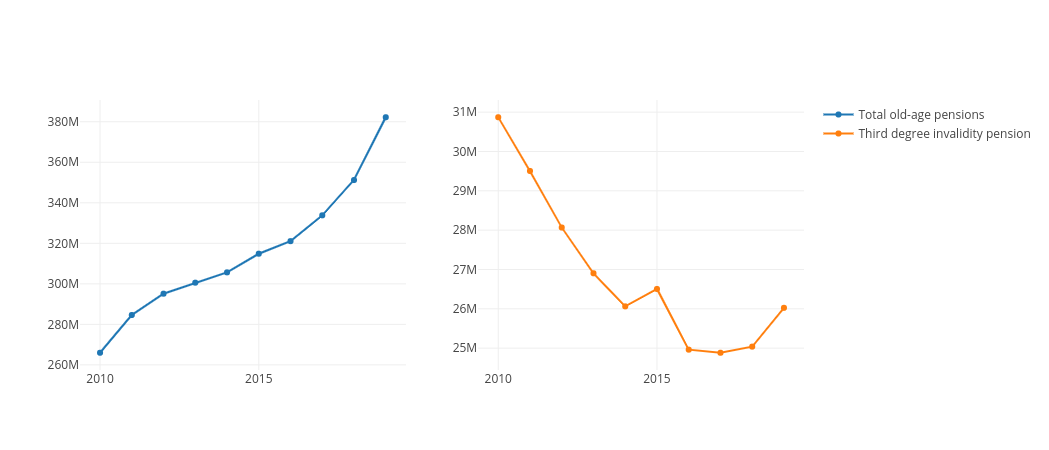
\includegraphics[width=\textwidth]{img/expenses.png}
\caption{Expenditure of selected pension kinds over time}
\label{expenditure}
\end{figure}

\subsection{Appending the YAGO Data Set to the CZSO Data Cubes\label{jaur-yago}}

In this task the mining tasks were performed over the CZSO's data cube \textit{Job Applicants and Unemployment Rate}, from now on denoted as \textit{JAUR}, and the triples extracted from YAGO data set. The data cube contains dimensions of reference area (89 distinct dimension values constisting of 13 regions without Prague and 76 districts without Prague, meaning there are no data concerning Prague), reference period (years 2005 to 2013) and sex (male, female and total). Each observation in the cube contains multiple measures. All observations are assigned the measures of number of available job applicants (job applicants who have no objective obstacle to taking up a job, e.g. enrollment in retraining courses or serving a sentence) and unemployment rate. Observations concerning both sexes also contain the measures of all job applicants and number of vacancies.

The data cube had to be sliced along the dimensions of reference area and sex. The dimension of reference area was divided into regions and districts. It was considered to divide the dimension of sex by each dimension value, but there is no significant difference between the male and female values\footnote{\href{https://nvkp.github.io/diploma-thesis-code/data/jaur/SexDimension}{https://nvkp.github.io/diploma-thesis-code/data/jaur/SexDimension}}, so the dimension was divided into \textit{total} and \textit{by-sex} part. That makes 4 slices \footnote{\href{https://nvkp.github.io/diploma-thesis-code/data/jaur/slice-queries/}{https://nvkp.github.io/diploma-thesis-code/data/jaur/slice-queries/}} with \numprint{2403} observations ($3 \times 9 \times 89$) and \numprint{6408} measured values in total, here denoted as \textit{regions-total}, \textit{regions-by-sex},  \textit{districts-total} and \textit{districts-by-sex}

All the measured values were discretized\footnote{\href{https://nvkp.github.io/diploma-thesis-code/notebooks/jaur}{https://nvkp.github.io/diploma-thesis-code/notebooks/jaur}} equifrequently. The measures of the subcubes \textit{regions-total} and \textit{regions-by-sex} were discretized twice with interval counts of 5 and 10. The measures of the subcubes \textit{districts-total} and \textit{districts-by-sex} were discretized with interval counts of 10, 20 and 30.

The notebook \verb|jaur-yago.ipynb|\footnote{\href{https://nvkp.github.io/diploma-thesis-code/notebooks/jaur-yago}{https://nvkp.github.io/diploma-thesis-code/notebooks/jaur-yago}} contains the mining itself. The YAGO triples and data cube's triples were merged together with the appropriate reference area linking triples\footnote{\href{https://nvkp.github.io/diploma-thesis-code/data/linking/yagoCZSOLinking.ttl}{https://nvkp.github.io/diploma-thesis-code/data/linking/yagoCZSOLinking.ttl}}. A separate index (containing all the extracted YAGO triples, the reference area linking triples and only those triples from the \textit{JAUR} cube that belong to the subcube's observations) was created for each of the four subcubes. That way the lift measure calculated for the rules mined from the indices is not distorted because its denominator is not increased by inappropriate observations.

Just as in the previous example, a pattern had to be provided to the mining tasks, that generates rules assigning a particular interval of a measure for observations satisfying the rule's body. In this pattern a variable at the position of object with the predicate of \verb|refArea| appears in an atom that is enforced to bind to triples from the YAGO data set. The atoms of the YAGO are enforced only to be present. They are not prescribed any rigid structure in the rules. For a mining task working with such pattern the threshold of maximal rule's length can be declared that corresponds to the number of hops of the extracted YAGO triples (determining the maximal length of the atom \verb|chain| from YAGO) and the number of other atoms in the body and the head atom.

For fininishing the mining task in a reasonable time also a minimal support thresholds had to be declared. The support of the sought rules corresponds to the number of observations for which the rule is valid. The rules have to contain an atom achoring the observations' variable to a constant of a slice by the \verb|qb:dataSet| predicate to ensure that each rule relates to one and only slice. The slices of the \textit{JAUR} data cube contain a different number of observations, so if a too high minimal support threshold is declared, the potentionally accurate rules from the a smaller slices would be discarded. In \ref{expenses-wikidata} all the slices contain the same number of observations and the whole cube so small that no minimal support threshold had to be used. In this mining task the problem was avoided by creating 4 distinct patterns that anchor the observations to each slice. These patterns are then appended to a separate mining tasks for each subcube with different minimal support thresholds.

\begin{figure}[h]
\begin{lstlisting}[language = scala, caption={Pattern definition for the slice \textit{districts-by-sex}}, label={jaurYagoPatterns},captionpos=b, escapeinside={(*@}{@*)}]
val districtBySexPattern = (
    AtomPattern(subject='b',graph=uri("yago"))&:
    AtomPattern(subject='a',predicate=refArea,`object`='b',graph=uri("czso"))&:
    AtomPattern(subject='a',predicate=qbDataSet,`object`=districtBySexSlice,graph=uri("czso"))
    =>: 
    AtomPattern(subject='a',predicate=oneOfMeasures, graph = uri("czso"))
)
\end{lstlisting}
\end{figure}

The smallest slice is \verb|jaur-regions-total| with only \numprint{117} observations (9 years of 13 regions). Let's assume there is a rule that can be inferred from this data that predicts a certain measure value to be in a certain interval given a certain characteristic of the reference area of the observation. Not to describe only one specific region, there have to be at least two regions satisfying the rule. If the rule had the confidence of 1 its support would be \numprint{18} (9~years~$\times$~2~regions). A rule with confidence of 0,5 would have half the support. Less confident rules with support of 9 or higher support would \textit{cover} more regions. So the minimal support for each mining task corresponding to single slice was given as the number of observations in the slice divided by number of observations for a distinct reference area. For the district slices such designated threshold would however not restrict the search space to finish the procedure in a reasonable time so for these two mining tasks with largest number of observations the number was multiplied by 3 (We demand \textit{half confident} rules to concern at least 6 districts).

\begin{figure}[h]
\begin{lstlisting}[language = scala, caption={Mining task definition for the slice \textit{districts-by-sex}}, label={jaurYagoTasks},captionpos=b, escapeinside={(*@}{@*)}]
val districtBySexTask = Amie()
    .addThreshold(Threshold.MinSupport(minSupport(districtBySexSlice)*3))
    .addThreshold(Threshold.MaxRuleLength(6))
    .addConstraint(constantsOnlyAtObject)
    .addPattern(districtBySexPattern)
\end{lstlisting}
\end{figure}

RDFRules API provides a constraint that can be appended to the mining task that eliminates atoms with a constant at the position of subject to be considered during the rule refinement. This shrinks the task's search space and contributes to shorter runtime when such atoms are not relevant for the particular pattern. In \ref{expenses-wikidata} this constraint could not be used since the second atom pattern's subject in the rule pattern was the constant of the Czech Republic's URI. It makes sense to add the constraint now.

Folows the description of the processing of each mining task's retrieved rule set. The used patterns do not prescribe a structure for each atom in a rule. The length of the rules can vary from 4 to 6 atoms. The patterns do not prevent the refining operators from appending an atom to the rule's body, whose subject variable represents a different observation than the one in the rule's head. That practically introduces a new \textit{unclosed} cube to the rule and invalidates it. Atoms with a new observation variable in those rules are connected through the variable of reference area. They all contain atom with the new variable at the position of subject, reference area dimension URI at the position of predicate and the variable of reference area at the position of object. All those rules were filtered out. Only those rules in the rule set, that have exactly one atom with reference area dimension URI at the position of predicate were kept for further processing.

\begin{figure}[h]
\begin{lstlisting}[language = scala, caption={Example of a rule with an unclosed body cube}, label={invalidRuleExample},captionpos=b, escapeinside={(*@}{@*)}]
(?c czso:pocetVolnychMist <[ 1222.0 ; 1608.5 )_ef20_19/20>) ^ (?c czso:refArea ?b) ^ (?b <http://schema.org/containedInPlace> yago:Moravian-Silesian_Region) ^ (?a czso:refArea ?b) ^ (?a qb:dataSet <jaur-districts-total>) -> (?a czso:neumisteniUchazeciOZamestnani <[ 9877.0 ; 26549.0 ]_ef10_10/10>) 

| support: 30, headCoverage: 0.014619883040935672, confidence: 0.7142857142857143, pcaConfidence: 0.7142857142857143, lift: 6.979591836734694, headConfidence: 0.1023391812865497, headSize: 2052, bodySize: 42, pcaBodySize: 42
\end{lstlisting}
\end{figure}

There is apparently a correlation between the cube's measures (available applicants is a subset of all job applicants, lower unemployment rate corresponds to lower number of vacancies). The algorithm tends to create evident rules in the sense of \textit{if there is a lower unemployment rate in the area, there is a lower number of applicants registered at the Labor Office}. Not to bother with this kind of rules, the rules with a measure URI at the position of predicate in any atom in the rule's body were filtered out as well. 

\begin{figure}[h]
\begin{lstlisting}[language = scala, caption={Example of an rule describing the correlation of measures}, label={invalidRuleExample2},captionpos=b, escapeinside={(*@}{@*)}]
(?a czso:dosazitelniNeumisteniUchazeciOZamestnani <[ 9639.0 ; 25767.0 ]_ef10_10/10>) ^ (?b <http://schema.org/containedInPlace> yago:Moravian-Silesian_Region) ^ (?a czso:refArea ?b) ^ (?a qb:dataSet <jaur-districts-total>) -> (?a czso:neumisteniUchazeciOZamestnani <[ 9877.0 ; 26549.0 ]_ef10_10/10>) 

| support: 30, headCoverage: 0.014619883040935672, confidence: 1.0, pcaConfidence: 1.0, lift: 9.771428571428572, headConfidence: 0.1023391812865497, headSize: 2052, bodySize: 30, pcaBodySize: 30
\end{lstlisting}
\end{figure}

The lift and confidence were computed for the remaining rules in the rule sets (each for every subcube). All rules with the lift value lower than 1 and the confidence value lower than 0,5 were filtered out. On the remaining rules in the rule sets the DBScan clustering algorithm was used with parameters of minimum size of a cluster of 3, minimum similarity of rules in the same cluster of 85\%. The similarity was computed only based on the content of the rules, not their interest measures. \numprint{673} rules from the \textit{regions-total} ruleset were arranged into \numprint{75} clusters, \numprint{46} clusters emerged in the \numprint{457} rules of the \textit{regions-by-sex} rule set, \numprint{169} rules of \textit{districts-total} rule set were divided into \numprint{26} clusters, ant \numprint{320} rules of the \textit{districts-by-sex} rule set into \numprint{28} of them. From those four rule sets new rule sets were derived, which contain one rule for each cluster. All rule sets, \textit{raw}, filtered, clustered and pruned by clusters are published on a signpost page\footnote{\href{https://nvkp.github.io/diploma-thesis-code/rulesets/jaur-yago/}{https://nvkp.github.io/diploma-thesis-code/rulesets/jaur-yago/}} in the repository's Github Pages.

\subsection{Relation Between Measures from Different Data Cubes}

This section describes the demonstration of how the AMIE algorithm can be used to mine relations of measures from multiple data cubes described in \ref{morecubes}. The mining was performed on a cube published by CZSO containing average and median salaries for the regions in Czech Republic, here denoted as \textit{Salaries} and the CSSA's \textit{Pensions} cube mentioned in \ref{cssa}. The \textit{Salaries} cube is structured into 3 dimensions. The dimension of sex consists of 3 distinct values of male, female and both sexes. The dimension of reference area has 14 distinct values for 13 regions and Prague. The dimension of reference period contains 3 distinct values, meaning the data covers only three years, from 2010 to 2012. Each observation in the cube is assigned two measures of the average and the median salary. The cube had to be cut to 3 subcubes\footnote{\href{https://nvkp.github.io/diploma-thesis-code/data/salaries/slice-queries}{https://nvkp.github.io/diploma-thesis-code/data/salaries/slice-queries}} for each value of the dimension of sex, because the measures assigned to each value's observations were assumed incommensurable\footnote{\href{https://nvkp.github.io/diploma-thesis-code/data/salaries/SexDimension}{https://nvkp.github.io/diploma-thesis-code/data/salaries/SexDimension}}. Each of the subcubes\footnote{\href{https://nvkp.github.io/diploma-thesis-code/data/salaries}{https://nvkp.github.io/diploma-thesis-code/data/salaries}} contains 42 observations. Each measure was discretized\footnote{\href{https://nvkp.github.io/diploma-thesis-code/notebooks/salaries}{https://nvkp.github.io/diploma-thesis-code/notebooks/salaries}} four times with the interval counts of 2, 3, 5 and 7.

The \textit{Pensions} cube also contains statistics for individual districts and the whole state but those observations could be omitted, because they would not appear in the rules, since the \textit{Salaries} cube does not share those reference area dimension values. The same goes for its dimension of reference area. Only the years intersecting the \textit{Salaries} cube are useful. The filtered cube was cut\footnote{\href{https://nvkp.github.io/diploma-thesis-code/data/pensions/slice-queries}{https://nvkp.github.io/diploma-thesis-code/data/pensions/slice-queries}} along the dimensions of pension kind with 37 distinct values and sex with 3 distinct values. For each combination of pension kind and sex dimension value a subcube was created so the total number of used subcubes\footnote{\href{https://nvkp.github.io/diploma-thesis-code/data/pensions}{https://nvkp.github.io/diploma-thesis-code/data/pensions}} is 111. Those subcubes contain the same number of observations as the \textit{Salaries} subcubes. The \textit{Pensions} cube contains three measures: the average amount of pension, the average age, and the number of persons but each observation is assigned only one measure, so there are exactly three observations for each combination of pension kind\footnote{This is valid for the filtered observations used for this task. The observations for the years before 2010 use a different pensions scheme.}, reference area, reference period and sex. That has an impact on the lift measure and standard confidence (not on the PCA confidence thoughl), when the rule predicts an interval for the observation in this cube. The lift is overestimated and the standard confidence is underestimated. Each measure was discretized twice with interval counts of 2 and 3.

The discretization of the \textit{Pensions} cube and the mining itself is contained in notebook \verb|pensions-salaries.ipynb|\footnote{\href{https://nvkp.github.io/diploma-thesis-code/notebooks/pensions-salaries}{https://nvkp.github.io/diploma-thesis-code/notebooks/pensions-salaries}}. Three different instances of index were created. Each index was constructed from the triples of one of the \textit{Salaries} subcubes, 37 \textit{Pensions} subcubes with the same sex dimension value as the \textit{Salaries} subcube and the linking $owl:sameAs$ triples for reference area, sex and reference period. Two rule pattern were defined. One for the rules that predict an interval for an observation from one of the \textit{Pensions} subcubes based on the values in the \textit{Salaries} subcube and the seconds defines the shape of rules that predict an interval for an observation in the \textit{Salaries} subcube based on the values in one of the \textit{Pensions subcubes}.

\begin{figure}[h]
\begin{lstlisting}[language = scala, caption={Pattern definitions for relation between cubes}, label={jaurYagoPatterns},captionpos=b, escapeinside={(*@}{@*)}]
val salariesPensionsPattern: RulePattern = (
    AtomPattern(subject = 'c', predicate = oneOfSalariesMeasures, `object` = AnyConstant) &:
    AtomPattern(subject = 'c', predicate = czsoRefPeriod, `object` = 'd') &:
    AtomPattern(subject = 'a', predicate = cssaRefPeriod, `object` = 'd') &:
    AtomPattern(subject = 'c', predicate = qbDataSet, `object` = AnyConstant) &:
    AtomPattern(subject = 'c', predicate = czsoRefArea, `object` = 'b') &:
    AtomPattern(subject = 'a', predicate = cssaRefArea, `object` = 'b') &:
    AtomPattern(subject = 'a', predicate = cssaPensionKind, `object` = AnyConstant) &:
    AtomPattern(subject = 'a', predicate = qbDataSet, `object` = AnyConstant)
    =>:
    AtomPattern(subject = 'a', predicate = oneOfPensionsMeasures)
)

val pensionsSalariesPattern: RulePattern = (
    AtomPattern(subject = 'c', predicate = oneOfPensionsMeasures, `object` = AnyConstant) &:
    AtomPattern(subject = 'c', predicate = cssaPensionKind, `object` = AnyConstant) &:
    AtomPattern(subject = 'a', predicate = czsoRefPeriod, `object` = 'd') &:
    AtomPattern(subject = 'c', predicate = cssaRefPeriod, `object` = 'd') &:
    AtomPattern(subject = 'c', predicate = qbDataSet, `object` = AnyConstant) &:
    AtomPattern(subject = 'c', predicate = cssaRefArea, `object` = 'b') &:
    AtomPattern(subject = 'a', predicate = czsoRefArea, `object` = 'b') &:
    AtomPattern(subject = 'a', predicate = qbDataSet, `object` = AnyConstant)
    =>:
    AtomPattern(subject = 'a', predicate = oneOfSalariesMeasures)
)
\end{lstlisting}
\end{figure}

Application of these rule patterns with the maximum rule length results only in rules where both cubes' dimensions are closed. For each combination of rule pattern and index the algorithm was invoked with no minimal support threshold and maximum rule length corresponding to the length of the rule patterns. Each of the 6 rule sets was filtered to so that only the perfect rules remained. Those rules were sorted descendantly by support. A signpost\footnote{\href{https://nvkp.github.io/diploma-thesis-code/rulesets/pensions-salaries/}{https://nvkp.github.io/diploma-thesis-code/rulesets/pensions-salaries/}} page in the repository provides link to those exported rule sets. The rules containing broader intervals have higher support than the rules with narrower intervals. The listing \ref{highlowsupport} shows one of the rules with the highest support and one one of the rules with the lowest support.

\begin{figure}[h]
\begin{lstlisting}[language = scala, caption={Two of the resulting perfect rules}, label={highlowsupport},captionpos=b, escapeinside={(*@}{@*)}]
(?c czso:medianMzdy <[ 19229.0 ; 21214.0 )_ef2_1/2>) ^ (?c czso:refPeriod ?d) ^ (?a cssz-dimension:refPeriod ?d) ^ (?c qb:dataSet <salaries-total>) ^ (?c czso:refArea ?b) ^ (?a cssz-dimension:refArea ?b) ^ (?a cssz-dimension:druh-duchodu <https://data.cssz.cz/resource/pension-kind/PK_V_total_2010>) ^ (?a qb:dataSet <pensions-by-region-total-PK_V_total>) -> (?a <https://data.cssz.cz/ontology/measure/prumerna-vyse-duchodu-v-kc> <[ 10506.559275967385 ; 11475.861138653103 )_ef3_1/3>) 
| support: 21, headCoverage: 0.002027027027027027, confidence: 0.3333333333333333, pcaConfidence: 1.0, lift: 37.53623188405797, headConfidence: 0.00888030888030888, headSize: 10360, bodySize: 63, pcaBodySize: 21

(?c czso:medianMzdy <[ 22602.0 ; 28392.0 ]_ef7_7/7>) ^ (?c czso:refPeriod ?d) ^ (?a cssz-dimension:refPeriod ?d) ^ (?c qb:dataSet <salaries-total>) ^ (?c czso:refArea ?b) ^ (?a cssz-dimension:refArea ?b) ^ (?a cssz-dimension:druh-duchodu <https://data.cssz.cz/resource/pension-kind/PK_S_2010>) ^ (?a qb:dataSet <pensions-by-region-total-PK_S>) -> (?a <https://data.cssz.cz/ontology/measure/prumerny-vek> <[ 68.24930566713338 ; 70.01816377599448 )_ef3_1/3>) 
| support: 6, headCoverage: 5.791505791505791E-4, confidence: 0.3333333333333333, pcaConfidence: 1.0, lift: 38.37037037037037, headConfidence: 0.008687258687258687, headSize: 10360, bodySize: 18, pcaBodySize: 6
\end{lstlisting}
\end{figure}

The first rules states that the regions with a lower median salary (half of all regions) are also regions with a lower widow's and widower's pension. That makes sense considering that the widow's and widower's pensions are calculated based on the old age pension of the deceased partner and the old age pension of the partner was partly dependant on his or her salary. The second rule states that the two regions with the highest median salary are also regions with a lower average age of people receiving the old age pension. Note that the standard confidence is a third of the PCA confidence. That is because also the observation not assigned to the predicted measure are considered counterexamples and not only the third of them with the correct measure.

\begin{figure}[h]
\begin{lstlisting}[language = scala, caption={Example of two \textit{mirroring} rules}, label={mirroringrules},captionpos=b, escapeinside={(*@}{@*)}]
(?c czso:prumernaMzda <[ 26722.0 ; 27860.0 )_ef5_4/5>) ^ (?c czso:refPeriod ?d) ^ (?a cssz-dimension:refPeriod ?d) ^ (?c qb:dataSet <salaries-male>) ^ (?c czso:refArea ?b) ^ (?a cssz-dimension:refArea ?b) ^ (?a cssz-dimension:druh-duchodu <https://data.cssz.cz/resource/pension-kind/PK_ID_2010>) ^ (?a qb:dataSet <pensions-by-region-male-PK_ID>) -> (?a <https://data.cssz.cz/ontology/measure/prumerny-vek> <[ 48.615229885057474 ; 50.58006905532994 )_ef2_1/2>)
| support: 9, headCoverage: 8.687258687258687E-4, confidence: 0.3333333333333333, pcaConfidence: 1.0, lift: 24.666666666666664, headConfidence: 0.013513513513513514, headSize: 10360, bodySize: 27, pcaBodySize: 9
    
(?c <https://data.cssz.cz/ontology/measure/prumerny-vek> <[ 48.615229885057474 ; 50.58006905532994 )_ef2_1/2>) ^ (?c cssz-dimension:druh-duchodu <https://data.cssz.cz/resource/pension-kind/PK_ID_2010>) ^ (?a czso:refPeriod ?d) ^ (?c cssz-dimension:refPeriod ?d) ^ (?c qb:dataSet <pensions-by-region-male-PK_ID>) ^ (?c cssz-dimension:refArea ?b) ^ (?a czso:refArea ?b) ^ (?a qb:dataSet <salaries-male>) -> (?a czso:prumernaMzda <[ 26722.0 ; 27860.0 )_ef5_4/5>) 
| support: 9, headCoverage: 0.05357142857142857, confidence: 0.28125, pcaConfidence: 0.28125, lift: 1.3125, headConfidence: 0.21428571428571427, headSize: 168, bodySize: 32, pcaBodySize: 32
\end{lstlisting}
\end{figure}

The unfiltered rule sets generated from the same index but according to a different rule pattern have the same number of rules. That means that the rules are \textit{mirroring} each other and stating that either $A$ \textit{is associated with} $B$ or $A$ \textit{is associated with} $B$. An example of those mirroring rules is shown in the listing \ref{mirroringrules}.

The rules have the same support but a different confidence. The average salary in the range of \numprint{26722} CZK to \numprint{27860} CZK strongly implies a lower half of the average age of people receiving the second degree disability pension, but it does work the other way around. The second rule's confidence measures have the same value, because the \textit{Salaries} assigns all both measures to a single observation.